\documentclass[1p]{elsarticle_modified}
%\bibliographystyle{elsarticle-num}

%\usepackage[colorlinks]{hyperref}
%\usepackage{abbrmath_seonhwa} %\Abb, \Ascr, \Acal ,\Abf, \Afrak
\usepackage{amsfonts}
\usepackage{amssymb}
\usepackage{amsmath}
\usepackage{amsthm}
\usepackage{scalefnt}
\usepackage{amsbsy}
\usepackage{kotex}
\usepackage{caption}
\usepackage{subfig}
\usepackage{color}
\usepackage{graphicx}
\usepackage{xcolor} %% white, black, red, green, blue, cyan, magenta, yellow
\usepackage{float}
\usepackage{setspace}
\usepackage{hyperref}

\usepackage{tikz}
\usetikzlibrary{arrows}

\usepackage{multirow}
\usepackage{array} % fixed length table
\usepackage{hhline}

%%%%%%%%%%%%%%%%%%%%%
\makeatletter
\renewcommand*\env@matrix[1][\arraystretch]{%
	\edef\arraystretch{#1}%
	\hskip -\arraycolsep
	\let\@ifnextchar\new@ifnextchar
	\array{*\c@MaxMatrixCols c}}
\makeatother %https://tex.stackexchange.com/questions/14071/how-can-i-increase-the-line-spacing-in-a-matrix
%%%%%%%%%%%%%%%

\usepackage[normalem]{ulem}

\newcommand{\msout}[1]{\ifmmode\text{\sout{\ensuremath{#1}}}\else\sout{#1}\fi}
%SOURCE: \msout is \stkout macro in https://tex.stackexchange.com/questions/20609/strikeout-in-math-mode

\newcommand{\cancel}[1]{
	\ifmmode
	{\color{red}\msout{#1}}
	\else
	{\color{red}\sout{#1}}
	\fi
}

\newcommand{\add}[1]{
	{\color{blue}\uwave{#1}}
}

\newcommand{\replace}[2]{
	\ifmmode
	{\color{red}\msout{#1}}{\color{blue}\uwave{#2}}
	\else
	{\color{red}\sout{#1}}{\color{blue}\uwave{#2}}
	\fi
}

\newcommand{\Sol}{\mathcal{S}} %segment
\newcommand{\D}{D} %diagram
\newcommand{\A}{\mathcal{A}} %arc


%%%%%%%%%%%%%%%%%%%%%%%%%%%%%5 test

\def\sl{\operatorname{\textup{SL}}(2,\Cbb)}
\def\psl{\operatorname{\textup{PSL}}(2,\Cbb)}
\def\quan{\mkern 1mu \triangleright \mkern 1mu}

\theoremstyle{definition}
\newtheorem{thm}{Theorem}[section]
\newtheorem{prop}[thm]{Proposition}
\newtheorem{lem}[thm]{Lemma}
\newtheorem{ques}[thm]{Question}
\newtheorem{cor}[thm]{Corollary}
\newtheorem{defn}[thm]{Definition}
\newtheorem{exam}[thm]{Example}
\newtheorem{rmk}[thm]{Remark}
\newtheorem{alg}[thm]{Algorithm}

\newcommand{\I}{\sqrt{-1}}
\begin{document}

%\begin{frontmatter}
%
%\title{Boundary parabolic representations of knots up to 8 crossings}
%
%%% Group authors per affiliation:
%\author{Yunhi Cho} 
%\address{Department of Mathematics, University of Seoul, Seoul, Korea}
%\ead{yhcho@uos.ac.kr}
%
%
%\author{Seonhwa Kim} %\fnref{s_kim}}
%\address{Center for Geometry and Physics, Institute for Basic Science, Pohang, 37673, Korea}
%\ead{ryeona17@ibs.re.kr}
%
%\author{Hyuk Kim}
%\address{Department of Mathematical Sciences, Seoul National University, Seoul 08826, Korea}
%\ead{hyukkim@snu.ac.kr}
%
%\author{Seokbeom Yoon}
%\address{Department of Mathematical Sciences, Seoul National University, Seoul, 08826,  Korea}
%\ead{sbyoon15@snu.ac.kr}
%
%\begin{abstract}
%We find all boundary parabolic representation of knots up to 8 crossings.
%
%\end{abstract}
%\begin{keyword}
%    \MSC[2010] 57M25 
%\end{keyword}
%
%\end{frontmatter}

%\linenumbers
%\tableofcontents
%
\newcommand\colored[1]{\textcolor{white}{\rule[-0.35ex]{0.8em}{1.4ex}}\kern-0.8em\color{red} #1}%
%\newcommand\colored[1]{\textcolor{white}{ #1}\kern-2.17ex	\textcolor{white}{ #1}\kern-1.81ex	\textcolor{white}{ #1}\kern-2.15ex\color{red}#1	}

{\Large $\underline{12n_{0717}~(K12n_{0717})}$}

\setlength{\tabcolsep}{10pt}
\renewcommand{\arraystretch}{1.6}
\vspace{1cm}\begin{tabular}{m{100pt}>{\centering\arraybackslash}m{274pt}}
\multirow{5}{120pt}{
	\centering
	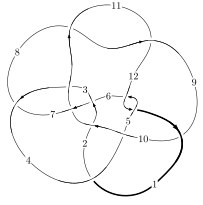
\includegraphics[width=112pt]{../../../GIT/diagram.site/Diagrams/png/2806_12n_0717.png}\\
\ \ \ A knot diagram\footnotemark}&
\allowdisplaybreaks
\textbf{Linearized knot diagam} \\
\cline{2-2}
 &
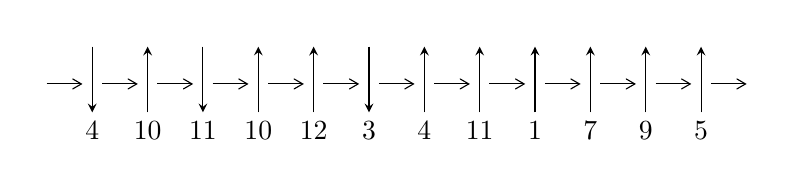
\begin{tikzpicture}[x=20pt, y=17pt]
	% nodes
	\node (C0) at (0, 0) {};
	\node (C1) at (1, 0) {};
	\node (C1U) at (1, +1) {};
	\node (C1D) at (1, -1) {4};

	\node (C2) at (2, 0) {};
	\node (C2U) at (2, +1) {};
	\node (C2D) at (2, -1) {10};

	\node (C3) at (3, 0) {};
	\node (C3U) at (3, +1) {};
	\node (C3D) at (3, -1) {11};

	\node (C4) at (4, 0) {};
	\node (C4U) at (4, +1) {};
	\node (C4D) at (4, -1) {10};

	\node (C5) at (5, 0) {};
	\node (C5U) at (5, +1) {};
	\node (C5D) at (5, -1) {12};

	\node (C6) at (6, 0) {};
	\node (C6U) at (6, +1) {};
	\node (C6D) at (6, -1) {3};

	\node (C7) at (7, 0) {};
	\node (C7U) at (7, +1) {};
	\node (C7D) at (7, -1) {4};

	\node (C8) at (8, 0) {};
	\node (C8U) at (8, +1) {};
	\node (C8D) at (8, -1) {11};

	\node (C9) at (9, 0) {};
	\node (C9U) at (9, +1) {};
	\node (C9D) at (9, -1) {1};

	\node (C10) at (10, 0) {};
	\node (C10U) at (10, +1) {};
	\node (C10D) at (10, -1) {7};

	\node (C11) at (11, 0) {};
	\node (C11U) at (11, +1) {};
	\node (C11D) at (11, -1) {9};

	\node (C12) at (12, 0) {};
	\node (C12U) at (12, +1) {};
	\node (C12D) at (12, -1) {5};
	\node (C13) at (13, 0) {};

	% arrows
	\draw[->,>={angle 60}]
	(C0) edge (C1) (C1) edge (C2) (C2) edge (C3) (C3) edge (C4) (C4) edge (C5) (C5) edge (C6) (C6) edge (C7) (C7) edge (C8) (C8) edge (C9) (C9) edge (C10) (C10) edge (C11) (C11) edge (C12) (C12) edge (C13) ;	\draw[->,>=stealth]
	(C1U) edge (C1D) (C2D) edge (C2U) (C3U) edge (C3D) (C4D) edge (C4U) (C5D) edge (C5U) (C6U) edge (C6D) (C7D) edge (C7U) (C8D) edge (C8U) (C9D) edge (C9U) (C10D) edge (C10U) (C11D) edge (C11U) (C12D) edge (C12U) ;
	\end{tikzpicture} \\
\hhline{~~} \\& 
\textbf{Solving Sequence} \\ \cline{2-2} 
 &
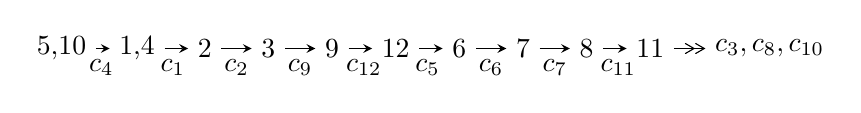
\begin{tikzpicture}[x=23pt, y=7pt]
	% node
	\node (A0) at (-1/8, 0) {5,10};
	\node (A1) at (17/16, 0) {1,4};
	\node (A2) at (17/8, 0) {2};
	\node (A3) at (25/8, 0) {3};
	\node (A4) at (33/8, 0) {9};
	\node (A5) at (41/8, 0) {12};
	\node (A6) at (49/8, 0) {6};
	\node (A7) at (57/8, 0) {7};
	\node (A8) at (65/8, 0) {8};
	\node (A9) at (73/8, 0) {11};
	\node (C1) at (1/2, -1) {$c_{4}$};
	\node (C2) at (13/8, -1) {$c_{1}$};
	\node (C3) at (21/8, -1) {$c_{2}$};
	\node (C4) at (29/8, -1) {$c_{9}$};
	\node (C5) at (37/8, -1) {$c_{12}$};
	\node (C6) at (45/8, -1) {$c_{5}$};
	\node (C7) at (53/8, -1) {$c_{6}$};
	\node (C8) at (61/8, -1) {$c_{7}$};
	\node (C9) at (69/8, -1) {$c_{11}$};
	\node (A10) at (11, 0) {$c_{3},c_{8},c_{10}$};

	% edge
	\draw[->,>=stealth]	
	(A0) edge (A1) (A1) edge (A2) (A2) edge (A3) (A3) edge (A4) (A4) edge (A5) (A5) edge (A6) (A6) edge (A7) (A7) edge (A8) (A8) edge (A9) ;
	\draw[->>,>={angle 60}]	
	(A9) edge (A10);
\end{tikzpicture} \\ 

\end{tabular} \\

\footnotetext{
The image of knot diagram is generated by the software ``\textbf{Draw programme}" developed by Andrew Bartholomew(\url{http://www.layer8.co.uk/maths/draw/index.htm\#Running-draw}), where we modified some parts for our purpose(\url{https://github.com/CATsTAILs/LinksPainter}).
}\phantom \\ \newline 
\centering \textbf{Ideals for irreducible components\footnotemark of $X_{\text{par}}$} 
 
\begin{align*}
I^u_{1}&=\langle 
25879 u^{15}-46049 u^{14}+\cdots+675712 b-1063104,\\
\phantom{I^u_{1}}&\phantom{= \langle  }463377 u^{15}-1801209 u^{14}+\cdots+9459968 a-26845656,\;u^{16}-3 u^{15}+\cdots-32 u-16\rangle \\
I^u_{2}&=\langle 
56993 u^{13} a+77423 u^{13}+\cdots+148181 a+443926,\\
\phantom{I^u_{2}}&\phantom{= \langle  }-5240829 u^{13} a-8288009 u^{13}+\cdots-52771818 a+2325177,\\
\phantom{I^u_{2}}&\phantom{= \langle  }u^{14}+u^{13}+10 u^{12}+8 u^{11}+36 u^{10}+22 u^9+61 u^8+34 u^7+73 u^6+54 u^5+82 u^4+53 u^3+43 u^2+20 u+11\rangle \\
I^u_{3}&=\langle 
31 u^{15}-15 u^{14}+\cdots+92 b-472,\;-577 u^{15}+3333 u^{14}+\cdots+9292 a+191294,\\
\phantom{I^u_{3}}&\phantom{= \langle  }u^{16}+11 u^{14}+54 u^{12}+160 u^{10}+329 u^8+496 u^6+526 u^4+343 u^2+101\rangle \\
\\
I^v_{1}&=\langle 
a,\;- v^2+b-3 v-1,\;v^3+3 v^2+2 v+1\rangle \\
\end{align*}
\raggedright * 4 irreducible components of $\dim_{\mathbb{C}}=0$, with total 63 representations.\\
\footnotetext{All coefficients of polynomials are rational numbers. But the coefficients are sometimes approximated in decimal forms when there is not enough margin.}
\newpage
\renewcommand{\arraystretch}{1}
\centering \section*{I. $I^u_{1}= \langle 2.59\times10^{4} u^{15}-4.60\times10^{4} u^{14}+\cdots+6.76\times10^{5} b-1.06\times10^{6},\;4.63\times10^{5} u^{15}-1.80\times10^{6} u^{14}+\cdots+9.46\times10^{6} a-2.68\times10^{7},\;u^{16}-3 u^{15}+\cdots-32 u-16 \rangle$}
\flushleft \textbf{(i) Arc colorings}\\
\begin{tabular}{m{7pt} m{180pt} m{7pt} m{180pt} }
\flushright $a_{5}=$&$\begin{pmatrix}1\\0\end{pmatrix}$ \\
\flushright $a_{10}=$&$\begin{pmatrix}0\\u\end{pmatrix}$ \\
\flushright $a_{1}=$&$\begin{pmatrix}-0.0489829 u^{15}+0.190403 u^{14}+\cdots-2.28630 u+2.83782\\-0.0382989 u^{15}+0.0681489 u^{14}+\cdots+1.61772 u+1.57331\end{pmatrix}$ \\
\flushright $a_{4}=$&$\begin{pmatrix}1\\u^2\end{pmatrix}$ \\
\flushright $a_{2}=$&$\begin{pmatrix}-0.0363658 u^{15}+0.193159 u^{14}+\cdots-3.29721 u+1.95978\\-0.0226024 u^{15}-0.0410566 u^{14}+\cdots+3.11903 u+2.22303\end{pmatrix}$ \\
\flushright $a_{3}=$&$\begin{pmatrix}-0.0363658 u^{15}+0.193159 u^{14}+\cdots-3.29721 u+1.95978\\-0.0126172 u^{15}-0.00275582 u^{14}+\cdots+1.01091 u+0.878038\end{pmatrix}$ \\
\flushright $a_{9}=$&$\begin{pmatrix}-0.0877234 u^{15}+0.254037 u^{14}+\cdots-1.23991 u+4.49819\\-0.0395677 u^{15}+0.170191 u^{14}+\cdots-1.04092 u+0.176944\end{pmatrix}$ \\
\flushright $a_{12}=$&$\begin{pmatrix}-0.0106841 u^{15}+0.122254 u^{14}+\cdots-3.90403 u+1.26451\\-0.0382989 u^{15}+0.0681489 u^{14}+\cdots+1.61772 u+1.57331\end{pmatrix}$ \\
\flushright $a_{6}=$&$\begin{pmatrix}-0.0800201 u^{15}+0.250091 u^{14}+\cdots+1.11319 u-1.40403\\0.0910791 u^{15}-0.322836 u^{14}+\cdots+0.378447 u+0.00921990\end{pmatrix}$ \\
\flushright $a_{7}=$&$\begin{pmatrix}-0.0489829 u^{15}+0.190403 u^{14}+\cdots-2.28630 u+2.83782\\0.0126172 u^{15}+0.00275582 u^{14}+\cdots-1.01091 u-0.878038\end{pmatrix}$ \\
\flushright $a_{8}=$&$\begin{pmatrix}-0.0106841 u^{15}+0.122254 u^{14}+\cdots-3.90403 u+1.26451\\-0.00563321 u^{15}-0.00282644 u^{14}+\cdots+1.09780 u-0.130074\end{pmatrix}$ \\
\flushright $a_{11}=$&$\begin{pmatrix}0.0877234 u^{15}-0.254037 u^{14}+\cdots+1.23991 u-4.49819\\-0.0179562 u^{15}+0.0609672 u^{14}+\cdots+0.654917 u+0.323076\end{pmatrix}$\\&\end{tabular}
\flushleft \textbf{(ii) Obstruction class $= -1$}\\~\\
\flushleft \textbf{(iii) Cusp Shapes $= -\frac{3140595}{4729984} u^{15}+\frac{9339149}{4729984} u^{14}+\cdots+\frac{1984439}{1182496} u+\frac{1721569}{73906}$}\\~\\
\newpage\renewcommand{\arraystretch}{1}
\flushleft \textbf{(iv) u-Polynomials at the component}\newline \\
\begin{tabular}{m{50pt}|m{274pt}}
Crossings & \hspace{64pt}u-Polynomials at each crossing \\
\hline $$\begin{aligned}c_{1}\end{aligned}$$&$\begin{aligned}
&u^{16}- u^{15}+\cdots-11 u+1
\end{aligned}$\\
\hline $$\begin{aligned}c_{2}\end{aligned}$$&$\begin{aligned}
&u^{16}-2 u^{15}+\cdots+194 u-121
\end{aligned}$\\
\hline $$\begin{aligned}c_{3}\end{aligned}$$&$\begin{aligned}
&u^{16}- u^{15}+\cdots-19 u+7
\end{aligned}$\\
\hline $$\begin{aligned}c_{4}\end{aligned}$$&$\begin{aligned}
&u^{16}-3 u^{15}+\cdots-32 u-16
\end{aligned}$\\
\hline $$\begin{aligned}c_{5},c_{7},c_{12}\end{aligned}$$&$\begin{aligned}
&u^{16}+u^{15}+\cdots-4 u+4
\end{aligned}$\\
\hline $$\begin{aligned}c_{6}\end{aligned}$$&$\begin{aligned}
&u^{16}+7 u^{15}+\cdots-65 u+28
\end{aligned}$\\
\hline $$\begin{aligned}c_{8},c_{11}\end{aligned}$$&$\begin{aligned}
&u^{16}+3 u^{15}+\cdots+13 u-28
\end{aligned}$\\
\hline $$\begin{aligned}c_{9},c_{10}\end{aligned}$$&$\begin{aligned}
&u^{16}-2 u^{14}+\cdots+4 u^2-1
\end{aligned}$\\
\hline
\end{tabular}\\~\\
\newpage\renewcommand{\arraystretch}{1}
\flushleft \textbf{(v) Riley Polynomials at the component}\newline \\
\begin{tabular}{m{50pt}|m{274pt}}
Crossings & \hspace{64pt}Riley Polynomials at each crossing \\
\hline $$\begin{aligned}c_{1}\end{aligned}$$&$\begin{aligned}
&y^{16}-21 y^{15}+\cdots-131 y+1
\end{aligned}$\\
\hline $$\begin{aligned}c_{2}\end{aligned}$$&$\begin{aligned}
&y^{16}+26 y^{15}+\cdots-15614 y+14641
\end{aligned}$\\
\hline $$\begin{aligned}c_{3}\end{aligned}$$&$\begin{aligned}
&y^{16}-19 y^{15}+\cdots-501 y+49
\end{aligned}$\\
\hline $$\begin{aligned}c_{4}\end{aligned}$$&$\begin{aligned}
&y^{16}+23 y^{15}+\cdots-2304 y+256
\end{aligned}$\\
\hline $$\begin{aligned}c_{5},c_{7},c_{12}\end{aligned}$$&$\begin{aligned}
&y^{16}+19 y^{15}+\cdots-80 y+16
\end{aligned}$\\
\hline $$\begin{aligned}c_{6}\end{aligned}$$&$\begin{aligned}
&y^{16}-25 y^{15}+\cdots-33289 y+784
\end{aligned}$\\
\hline $$\begin{aligned}c_{8},c_{11}\end{aligned}$$&$\begin{aligned}
&y^{16}+y^{15}+\cdots-7169 y+784
\end{aligned}$\\
\hline $$\begin{aligned}c_{9},c_{10}\end{aligned}$$&$\begin{aligned}
&y^{16}-4 y^{15}+\cdots-8 y+1
\end{aligned}$\\
\hline
\end{tabular}\\~\\
\newpage\flushleft \textbf{(vi) Complex Volumes and Cusp Shapes}
$$\begin{array}{c|c|c}  
\text{Solutions to }I^u_{1}& \I (\text{vol} + \sqrt{-1}CS) & \text{Cusp shape}\\
 \hline 
\begin{aligned}
u &= \phantom{-}0.119335 + 1.038870 I \\
a &= -0.494008 - 1.094850 I \\
b &= \phantom{-}0.17992 + 1.59062 I\end{aligned}
 & -3.83744 - 3.93600 I & \phantom{-}2.87663 + 4.26125 I \\ \hline\begin{aligned}
u &= \phantom{-}0.119335 - 1.038870 I \\
a &= -0.494008 + 1.094850 I \\
b &= \phantom{-}0.17992 - 1.59062 I\end{aligned}
 & -3.83744 + 3.93600 I & \phantom{-}2.87663 - 4.26125 I \\ \hline\begin{aligned}
u &= -0.034961 + 1.296400 I \\
a &= -0.608719 + 0.180864 I \\
b &= -0.891539 - 0.005634 I\end{aligned}
 & -3.72865 + 1.11794 I & \phantom{-}3.47362 - 6.30090 I \\ \hline\begin{aligned}
u &= -0.034961 - 1.296400 I \\
a &= -0.608719 - 0.180864 I \\
b &= -0.891539 + 0.005634 I\end{aligned}
 & -3.72865 - 1.11794 I & \phantom{-}3.47362 + 6.30090 I \\ \hline\begin{aligned}
u &= -0.622483 + 0.254551 I \\
a &= \phantom{-}0.390738 + 0.662414 I \\
b &= -0.030479 + 1.183440 I\end{aligned}
 & -1.46484 + 2.93564 I & \phantom{-}5.07482 - 1.11353 I \\ \hline\begin{aligned}
u &= -0.622483 - 0.254551 I \\
a &= \phantom{-}0.390738 - 0.662414 I \\
b &= -0.030479 - 1.183440 I\end{aligned}
 & -1.46484 - 2.93564 I & \phantom{-}5.07482 + 1.11353 I \\ \hline\begin{aligned}
u &= \phantom{-}0.28607 + 1.44355 I \\
a &= \phantom{-}0.138612 - 0.552258 I \\
b &= -0.181437 + 0.590003 I\end{aligned}
 & \phantom{-}1.87947 - 1.24485 I & \phantom{-}11.40323 + 4.68247 I \\ \hline\begin{aligned}
u &= \phantom{-}0.28607 - 1.44355 I \\
a &= \phantom{-}0.138612 + 0.552258 I \\
b &= -0.181437 - 0.590003 I\end{aligned}
 & \phantom{-}1.87947 + 1.24485 I & \phantom{-}11.40323 - 4.68247 I \\ \hline\begin{aligned}
u &= \phantom{-}0.503828\phantom{ +0.000000I} \\
a &= \phantom{-}0.941502\phantom{ +0.000000I} \\
b &= \phantom{-}0.334619\phantom{ +0.000000I}\end{aligned}
 & \phantom{-}0.729058\phantom{ +0.000000I} & \phantom{-}13.6990\phantom{ +0.000000I} \\ \hline\begin{aligned}
u &= -0.382038\phantom{ +0.000000I} \\
a &= \phantom{-}3.33621\phantom{ +0.000000I} \\
b &= \phantom{-}0.692814\phantom{ +0.000000I}\end{aligned}
 & \phantom{-}6.53070\phantom{ +0.000000I} & \phantom{-}22.8110\phantom{ +0.000000I}\\
 \hline 
 \end{array}$$\newpage$$\begin{array}{c|c|c}  
\text{Solutions to }I^u_{1}& \I (\text{vol} + \sqrt{-1}CS) & \text{Cusp shape}\\
 \hline 
\begin{aligned}
u &= \phantom{-}0.03599 + 1.87656 I \\
a &= \phantom{-}0.554024 + 0.651219 I \\
b &= -0.12246 - 1.50429 I\end{aligned}
 & -15.1090 - 2.7222 I & \phantom{-}2.22525 + 1.87237 I \\ \hline\begin{aligned}
u &= \phantom{-}0.03599 - 1.87656 I \\
a &= \phantom{-}0.554024 - 0.651219 I \\
b &= -0.12246 + 1.50429 I\end{aligned}
 & -15.1090 + 2.7222 I & \phantom{-}2.22525 - 1.87237 I \\ \hline\begin{aligned}
u &= \phantom{-}1.25896 + 1.40167 I \\
a &= -0.587811 + 0.033755 I \\
b &= -0.566111 - 1.293200 I\end{aligned}
 & -5.72547 + 7.15671 I & \phantom{-}3.37598 - 8.21855 I \\ \hline\begin{aligned}
u &= \phantom{-}1.25896 - 1.40167 I \\
a &= -0.587811 - 0.033755 I \\
b &= -0.566111 + 1.293200 I\end{aligned}
 & -5.72547 - 7.15671 I & \phantom{-}3.37598 + 8.21855 I \\ \hline\begin{aligned}
u &= \phantom{-}0.39619 + 1.87970 I \\
a &= \phantom{-}0.718306 - 0.433411 I \\
b &= \phantom{-}0.59839 + 1.77105 I\end{aligned}
 & -15.9449 + 14.1335 I & \phantom{-}2.81526 - 6.31158 I \\ \hline\begin{aligned}
u &= \phantom{-}0.39619 - 1.87970 I \\
a &= \phantom{-}0.718306 + 0.433411 I \\
b &= \phantom{-}0.59839 - 1.77105 I\end{aligned}
 & -15.9449 - 14.1335 I & \phantom{-}2.81526 + 6.31158 I\\
 \hline 
 \end{array}$$\newpage\newpage\renewcommand{\arraystretch}{1}
\centering \section*{II. $I^u_{2}= \langle 5.70\times10^{4} a u^{13}+7.74\times10^{4} u^{13}+\cdots+1.48\times10^{5} a+4.44\times10^{5},\;-5.24\times10^{6} a u^{13}-8.29\times10^{6} u^{13}+\cdots-5.28\times10^{7} a+2.33\times10^{6},\;u^{14}+u^{13}+\cdots+20 u+11 \rangle$}
\flushleft \textbf{(i) Arc colorings}\\
\begin{tabular}{m{7pt} m{180pt} m{7pt} m{180pt} }
\flushright $a_{5}=$&$\begin{pmatrix}1\\0\end{pmatrix}$ \\
\flushright $a_{10}=$&$\begin{pmatrix}0\\u\end{pmatrix}$ \\
\flushright $a_{1}=$&$\begin{pmatrix}a\\-0.0750130 a u^{13}-0.101903 u^{13}+\cdots-0.195033 a-0.584286\end{pmatrix}$ \\
\flushright $a_{4}=$&$\begin{pmatrix}1\\u^2\end{pmatrix}$ \\
\flushright $a_{2}=$&$\begin{pmatrix}0.0750130 a u^{13}+0.101903 u^{13}+\cdots+1.19503 a+0.584286\\-0.224463 a u^{13}-0.244106 u^{13}+\cdots+0.0452147 a-0.589078\end{pmatrix}$ \\
\flushright $a_{3}=$&$\begin{pmatrix}0.0750130 a u^{13}+0.101903 u^{13}+\cdots+1.19503 a+0.584286\\-0.0750130 a u^{13}-0.101903 u^{13}+\cdots-0.195033 a-0.584286\end{pmatrix}$ \\
\flushright $a_{9}=$&$\begin{pmatrix}0.0975842 a u^{13}+0.0595029 u^{13}+\cdots+0.627079 a+0.991682\\-0.163468 a u^{13}-0.151136 u^{13}+\cdots-0.199622 a-1.64704\end{pmatrix}$ \\
\flushright $a_{12}=$&$\begin{pmatrix}0.0750130 a u^{13}+0.101903 u^{13}+\cdots+1.19503 a+0.584286\\-0.0750130 a u^{13}-0.101903 u^{13}+\cdots-0.195033 a-0.584286\end{pmatrix}$ \\
\flushright $a_{6}=$&$\begin{pmatrix}-0.00230200 a u^{13}+0.190411 u^{13}+\cdots-1.39365 a+0.990069\\0.0204495 a u^{13}-0.0406805 u^{13}+\cdots-0.334311 a-1.07057\end{pmatrix}$ \\
\flushright $a_{7}=$&$\begin{pmatrix}0.0570072 u^{13}-0.0405770 u^{12}+\cdots-a+0.574026\\-0.0750130 a u^{13}+0.0927235 u^{13}+\cdots-0.195033 a-0.654532\end{pmatrix}$ \\
\flushright $a_{8}=$&$\begin{pmatrix}-0.0750130 a u^{13}+0.0751547 u^{13}+\cdots-1.19503 a-1.15393\\0.0744365 a u^{13}+0.246160 u^{13}+\cdots-0.435280 a+1.14362\end{pmatrix}$ \\
\flushright $a_{11}=$&$\begin{pmatrix}0.0975842 a u^{13}+0.0187794 u^{13}+\cdots+0.627079 a+0.0745087\\0.0535514 a u^{13}-0.0354421 u^{13}+\cdots+1.01996 a+0.618570\end{pmatrix}$\\&\end{tabular}
\flushleft \textbf{(ii) Obstruction class $= -1$}\\~\\
\flushleft \textbf{(iii) Cusp Shapes $= \frac{4926}{30391} u^{13}-\frac{83536}{151955} u^{12}+\cdots-\frac{1805974}{151955} u-\frac{701964}{151955}$}\\~\\
\newpage\renewcommand{\arraystretch}{1}
\flushleft \textbf{(iv) u-Polynomials at the component}\newline \\
\begin{tabular}{m{50pt}|m{274pt}}
Crossings & \hspace{64pt}u-Polynomials at each crossing \\
\hline $$\begin{aligned}c_{1}\end{aligned}$$&$\begin{aligned}
&u^{28}-5 u^{27}+\cdots+1150 u+5663
\end{aligned}$\\
\hline $$\begin{aligned}c_{2}\end{aligned}$$&$\begin{aligned}
&u^{28}+u^{27}+\cdots+20378 u+5689
\end{aligned}$\\
\hline $$\begin{aligned}c_{3}\end{aligned}$$&$\begin{aligned}
&u^{28}-14 u^{26}+\cdots+40 u+13
\end{aligned}$\\
\hline $$\begin{aligned}c_{4}\end{aligned}$$&$\begin{aligned}
&(u^{14}+u^{13}+\cdots+20 u+11)^{2}
\end{aligned}$\\
\hline $$\begin{aligned}c_{5},c_{7},c_{12}\end{aligned}$$&$\begin{aligned}
&u^{28}-4 u^{27}+\cdots+52 u+4
\end{aligned}$\\
\hline $$\begin{aligned}c_{6}\end{aligned}$$&$\begin{aligned}
&(u^{14}-3 u^{13}+\cdots+9 u+1)^{2}
\end{aligned}$\\
\hline $$\begin{aligned}c_{8},c_{11}\end{aligned}$$&$\begin{aligned}
&(u^{14}-2 u^{13}+\cdots+10 u+19)^{2}
\end{aligned}$\\
\hline $$\begin{aligned}c_{9},c_{10}\end{aligned}$$&$\begin{aligned}
&u^{28}- u^{27}+\cdots-2 u+7
\end{aligned}$\\
\hline
\end{tabular}\\~\\
\newpage\renewcommand{\arraystretch}{1}
\flushleft \textbf{(v) Riley Polynomials at the component}\newline \\
\begin{tabular}{m{50pt}|m{274pt}}
Crossings & \hspace{64pt}Riley Polynomials at each crossing \\
\hline $$\begin{aligned}c_{1}\end{aligned}$$&$\begin{aligned}
&y^{28}-65 y^{27}+\cdots+1024529950 y+32069569
\end{aligned}$\\
\hline $$\begin{aligned}c_{2}\end{aligned}$$&$\begin{aligned}
&y^{28}+95 y^{27}+\cdots+1623868142 y+32364721
\end{aligned}$\\
\hline $$\begin{aligned}c_{3}\end{aligned}$$&$\begin{aligned}
&y^{28}-28 y^{27}+\cdots+5316 y+169
\end{aligned}$\\
\hline $$\begin{aligned}c_{4}\end{aligned}$$&$\begin{aligned}
&(y^{14}+19 y^{13}+\cdots+546 y+121)^{2}
\end{aligned}$\\
\hline $$\begin{aligned}c_{5},c_{7},c_{12}\end{aligned}$$&$\begin{aligned}
&y^{28}+22 y^{27}+\cdots-192 y+16
\end{aligned}$\\
\hline $$\begin{aligned}c_{6}\end{aligned}$$&$\begin{aligned}
&(y^{14}-25 y^{13}+\cdots+213 y+1)^{2}
\end{aligned}$\\
\hline $$\begin{aligned}c_{8},c_{11}\end{aligned}$$&$\begin{aligned}
&(y^{14}+6 y^{13}+\cdots+1572 y+361)^{2}
\end{aligned}$\\
\hline $$\begin{aligned}c_{9},c_{10}\end{aligned}$$&$\begin{aligned}
&y^{28}+5 y^{27}+\cdots+808 y+49
\end{aligned}$\\
\hline
\end{tabular}\\~\\
\newpage\flushleft \textbf{(vi) Complex Volumes and Cusp Shapes}
$$\begin{array}{c|c|c}  
\text{Solutions to }I^u_{2}& \I (\text{vol} + \sqrt{-1}CS) & \text{Cusp shape}\\
 \hline 
\begin{aligned}
u &= -0.608535 + 0.818694 I \\
a &= -0.411980 + 0.907499 I \\
b &= \phantom{-}0.06835 - 1.89797 I\end{aligned}
 & -6.55425 - 2.13545 I & -1.029851 + 0.927255 I \\ \hline\begin{aligned}
u &= -0.608535 + 0.818694 I \\
a &= -1.176640 + 0.343109 I \\
b &= -0.361633 + 1.267890 I\end{aligned}
 & -6.55425 - 2.13545 I & -1.029851 + 0.927255 I \\ \hline\begin{aligned}
u &= -0.608535 - 0.818694 I \\
a &= -0.411980 - 0.907499 I \\
b &= \phantom{-}0.06835 + 1.89797 I\end{aligned}
 & -6.55425 + 2.13545 I & -1.029851 - 0.927255 I \\ \hline\begin{aligned}
u &= -0.608535 - 0.818694 I \\
a &= -1.176640 - 0.343109 I \\
b &= -0.361633 - 1.267890 I\end{aligned}
 & -6.55425 + 2.13545 I & -1.029851 - 0.927255 I \\ \hline\begin{aligned}
u &= \phantom{-}0.867236 + 0.768486 I \\
a &= \phantom{-}0.660917 - 0.753698 I \\
b &= \phantom{-}0.417481 + 0.355557 I\end{aligned}
 & \phantom{-}1.07339 - 1.32380 I & \phantom{-}7.73703 - 5.74981 I \\ \hline\begin{aligned}
u &= \phantom{-}0.867236 + 0.768486 I \\
a &= \phantom{-}0.437028 + 0.279301 I \\
b &= -0.241912 + 0.857846 I\end{aligned}
 & \phantom{-}1.07339 - 1.32380 I & \phantom{-}7.73703 - 5.74981 I \\ \hline\begin{aligned}
u &= \phantom{-}0.867236 - 0.768486 I \\
a &= \phantom{-}0.660917 + 0.753698 I \\
b &= \phantom{-}0.417481 - 0.355557 I\end{aligned}
 & \phantom{-}1.07339 + 1.32380 I & \phantom{-}7.73703 + 5.74981 I \\ \hline\begin{aligned}
u &= \phantom{-}0.867236 - 0.768486 I \\
a &= \phantom{-}0.437028 - 0.279301 I \\
b &= -0.241912 - 0.857846 I\end{aligned}
 & \phantom{-}1.07339 + 1.32380 I & \phantom{-}7.73703 + 5.74981 I \\ \hline\begin{aligned}
u &= \phantom{-}0.166845 + 0.745853 I \\
a &= \phantom{-}1.198390 - 0.576968 I \\
b &= \phantom{-}0.58958 + 1.51898 I\end{aligned}
 & \phantom{-}0.78349 + 4.75239 I & \phantom{-}9.02300 - 5.96017 I \\ \hline\begin{aligned}
u &= \phantom{-}0.166845 + 0.745853 I \\
a &= -0.90241 + 1.32619 I \\
b &= -0.128235 + 0.168215 I\end{aligned}
 & \phantom{-}0.78349 + 4.75239 I & \phantom{-}9.02300 - 5.96017 I\\
 \hline 
 \end{array}$$\newpage$$\begin{array}{c|c|c}  
\text{Solutions to }I^u_{2}& \I (\text{vol} + \sqrt{-1}CS) & \text{Cusp shape}\\
 \hline 
\begin{aligned}
u &= \phantom{-}0.166845 - 0.745853 I \\
a &= \phantom{-}1.198390 + 0.576968 I \\
b &= \phantom{-}0.58958 - 1.51898 I\end{aligned}
 & \phantom{-}0.78349 - 4.75239 I & \phantom{-}9.02300 + 5.96017 I \\ \hline\begin{aligned}
u &= \phantom{-}0.166845 - 0.745853 I \\
a &= -0.90241 - 1.32619 I \\
b &= -0.128235 - 0.168215 I\end{aligned}
 & \phantom{-}0.78349 - 4.75239 I & \phantom{-}9.02300 + 5.96017 I \\ \hline\begin{aligned}
u &= -0.564009 + 0.438487 I \\
a &= -0.755998 + 0.580538 I \\
b &= -0.825125 - 0.177451 I\end{aligned}
 & -2.32511 - 1.81694 I & \phantom{-}2.43913 + 3.97393 I \\ \hline\begin{aligned}
u &= -0.564009 + 0.438487 I \\
a &= \phantom{-}1.174370 - 0.329537 I \\
b &= \phantom{-}0.126698 - 1.153290 I\end{aligned}
 & -2.32511 - 1.81694 I & \phantom{-}2.43913 + 3.97393 I \\ \hline\begin{aligned}
u &= -0.564009 - 0.438487 I \\
a &= -0.755998 - 0.580538 I \\
b &= -0.825125 + 0.177451 I\end{aligned}
 & -2.32511 + 1.81694 I & \phantom{-}2.43913 - 3.97393 I \\ \hline\begin{aligned}
u &= -0.564009 - 0.438487 I \\
a &= \phantom{-}1.174370 + 0.329537 I \\
b &= \phantom{-}0.126698 + 1.153290 I\end{aligned}
 & -2.32511 + 1.81694 I & \phantom{-}2.43913 - 3.97393 I \\ \hline\begin{aligned}
u &= -0.22941 + 1.46771 I \\
a &= -1.023950 - 0.634998 I \\
b &= -0.25347 + 1.40401 I\end{aligned}
 & -8.50378 - 4.79575 I & -8.7502 + 11.1583 I \\ \hline\begin{aligned}
u &= -0.22941 + 1.46771 I \\
a &= \phantom{-}0.405862 + 0.057348 I \\
b &= \phantom{-}2.70787 - 0.47109 I\end{aligned}
 & -8.50378 - 4.79575 I & -8.7502 + 11.1583 I \\ \hline\begin{aligned}
u &= -0.22941 - 1.46771 I \\
a &= -1.023950 + 0.634998 I \\
b &= -0.25347 - 1.40401 I\end{aligned}
 & -8.50378 + 4.79575 I & -8.7502 - 11.1583 I \\ \hline\begin{aligned}
u &= -0.22941 - 1.46771 I \\
a &= \phantom{-}0.405862 - 0.057348 I \\
b &= \phantom{-}2.70787 + 0.47109 I\end{aligned}
 & -8.50378 + 4.79575 I & -8.7502 - 11.1583 I\\
 \hline 
 \end{array}$$\newpage$$\begin{array}{c|c|c}  
\text{Solutions to }I^u_{2}& \I (\text{vol} + \sqrt{-1}CS) & \text{Cusp shape}\\
 \hline 
\begin{aligned}
u &= -0.20751 + 1.75492 I \\
a &= \phantom{-}0.579759 - 0.748808 I \\
b &= -0.11875 + 1.53558 I\end{aligned}
 & -15.7247 - 5.5362 I & \phantom{-}2.24093 + 2.42211 I \\ \hline\begin{aligned}
u &= -0.20751 + 1.75492 I \\
a &= \phantom{-}0.732938 + 0.492983 I \\
b &= \phantom{-}0.60418 - 1.81331 I\end{aligned}
 & -15.7247 - 5.5362 I & \phantom{-}2.24093 + 2.42211 I \\ \hline\begin{aligned}
u &= -0.20751 - 1.75492 I \\
a &= \phantom{-}0.579759 + 0.748808 I \\
b &= -0.11875 - 1.53558 I\end{aligned}
 & -15.7247 + 5.5362 I & \phantom{-}2.24093 - 2.42211 I \\ \hline\begin{aligned}
u &= -0.20751 - 1.75492 I \\
a &= \phantom{-}0.732938 - 0.492983 I \\
b &= \phantom{-}0.60418 + 1.81331 I\end{aligned}
 & -15.7247 + 5.5362 I & \phantom{-}2.24093 - 2.42211 I \\ \hline\begin{aligned}
u &= \phantom{-}0.07539 + 1.95612 I \\
a &= -0.602812 + 0.538409 I \\
b &= -0.34660 - 1.66417 I\end{aligned}
 & -9.87238 + 4.14557 I & -1.66007 - 2.24011 I \\ \hline\begin{aligned}
u &= \phantom{-}0.07539 + 1.95612 I \\
a &= \phantom{-}0.457249 + 0.003148 I \\
b &= -0.238434 - 0.063577 I\end{aligned}
 & -9.87238 + 4.14557 I & -1.66007 - 2.24011 I \\ \hline\begin{aligned}
u &= \phantom{-}0.07539 - 1.95612 I \\
a &= -0.602812 - 0.538409 I \\
b &= -0.34660 + 1.66417 I\end{aligned}
 & -9.87238 - 4.14557 I & -1.66007 + 2.24011 I \\ \hline\begin{aligned}
u &= \phantom{-}0.07539 - 1.95612 I \\
a &= \phantom{-}0.457249 - 0.003148 I \\
b &= -0.238434 + 0.063577 I\end{aligned}
 & -9.87238 - 4.14557 I & -1.66007 + 2.24011 I\\
 \hline 
 \end{array}$$\newpage\newpage\renewcommand{\arraystretch}{1}
\centering \section*{III. $I^u_{3}= \langle 31 u^{15}-15 u^{14}+\cdots+92 b-472,\;-577 u^{15}+3333 u^{14}+\cdots+9292 a+191294,\;u^{16}+11 u^{14}+\cdots+343 u^2+101 \rangle$}
\flushleft \textbf{(i) Arc colorings}\\
\begin{tabular}{m{7pt} m{180pt} m{7pt} m{180pt} }
\flushright $a_{5}=$&$\begin{pmatrix}1\\0\end{pmatrix}$ \\
\flushright $a_{10}=$&$\begin{pmatrix}0\\u\end{pmatrix}$ \\
\flushright $a_{1}=$&$\begin{pmatrix}0.0620964 u^{15}-0.358696 u^{14}+\cdots+1.99473 u-20.5870\\-0.336957 u^{15}+0.163043 u^{14}+\cdots-28.1196 u+5.13043\end{pmatrix}$ \\
\flushright $a_{4}=$&$\begin{pmatrix}1\\u^2\end{pmatrix}$ \\
\flushright $a_{2}=$&$\begin{pmatrix}0.246879 u^{15}+0.0760870 u^{14}+\cdots+23.8426 u+10.5109\\-0.478261 u^{15}-0.478261 u^{14}+\cdots-46.7826 u-38.7826\end{pmatrix}$ \\
\flushright $a_{3}=$&$\begin{pmatrix}0.246879 u^{15}+0.0760870 u^{14}+\cdots+23.8426 u+10.5109\\-0.184783 u^{15}-0.434783 u^{14}+\cdots-21.8478 u-31.0978\end{pmatrix}$ \\
\flushright $a_{9}=$&$\begin{pmatrix}-0.627206 u^{15}-0.391304 u^{14}+\cdots-41.2622 u-21.9130\\0.239130 u^{15}+0.336957 u^{14}+\cdots+15.6413 u+28.1196\end{pmatrix}$ \\
\flushright $a_{12}=$&$\begin{pmatrix}0.399053 u^{15}-0.521739 u^{14}+\cdots+30.1143 u-25.7174\\-0.336957 u^{15}+0.163043 u^{14}+\cdots-28.1196 u+5.13043\end{pmatrix}$ \\
\flushright $a_{6}=$&$\begin{pmatrix}0.243328 u^{15}-0.130435 u^{14}+\cdots+25.1461 u+4.44565\\-0.521739 u^{15}+0.369565 u^{14}+\cdots-49.2174 u+11.1957\end{pmatrix}$ \\
\flushright $a_{7}=$&$\begin{pmatrix}-0.0620964 u^{15}-0.358696 u^{14}+\cdots-1.99473 u-20.5870\\-0.184783 u^{15}+0.434783 u^{14}+\cdots-21.8478 u+31.0978\end{pmatrix}$ \\
\flushright $a_{8}=$&$\begin{pmatrix}-0.399053 u^{15}-0.521739 u^{14}+\cdots-30.1143 u-25.7174\\0.293478 u^{15}+0.706522 u^{14}+\cdots+12.1848 u+47.5652\end{pmatrix}$ \\
\flushright $a_{11}=$&$\begin{pmatrix}0.627206 u^{15}-0.391304 u^{14}+\cdots+41.2622 u-21.9130\\-0.695652 u^{15}+0.315217 u^{14}+\cdots-47.7065 u+11.4022\end{pmatrix}$\\&\end{tabular}
\flushleft \textbf{(ii) Obstruction class $= 1$}\\~\\
\flushleft \textbf{(iii) Cusp Shapes $= -\frac{2}{23} u^{14}-\frac{34}{23} u^{12}-\frac{220}{23} u^{10}-\frac{766}{23} u^8-\frac{1666}{23} u^6-\frac{2524}{23} u^4-\frac{2672}{23} u^2-\frac{1354}{23}$}\\~\\
\newpage\renewcommand{\arraystretch}{1}
\flushleft \textbf{(iv) u-Polynomials at the component}\newline \\
\begin{tabular}{m{50pt}|m{274pt}}
Crossings & \hspace{64pt}u-Polynomials at each crossing \\
\hline $$\begin{aligned}c_{1}\end{aligned}$$&$\begin{aligned}
&u^{16}-10 u^{15}+\cdots-602 u+79
\end{aligned}$\\
\hline $$\begin{aligned}c_{2}\end{aligned}$$&$\begin{aligned}
&u^{16}-2 u^{15}+\cdots+2 u+1
\end{aligned}$\\
\hline $$\begin{aligned}c_{3}\end{aligned}$$&$\begin{aligned}
&u^{16}+u^{15}+\cdots+4 u+1
\end{aligned}$\\
\hline $$\begin{aligned}c_{4}\end{aligned}$$&$\begin{aligned}
&u^{16}+11 u^{14}+\cdots+343 u^2+101
\end{aligned}$\\
\hline $$\begin{aligned}c_{5},c_{7}\end{aligned}$$&$\begin{aligned}
&u^{16}- u^{15}+\cdots-8 u+4
\end{aligned}$\\
\hline $$\begin{aligned}c_{6}\end{aligned}$$&$\begin{aligned}
&(u^8-4 u^7+4 u^6+u^5-4 u^4+4 u^3+4 u^2- u-1)^2
\end{aligned}$\\
\hline $$\begin{aligned}c_{8}\end{aligned}$$&$\begin{aligned}
&(u^8+2 u^7- u^6-3 u^5-2 u^4-3 u^3+u^2+5 u+1)^2
\end{aligned}$\\
\hline $$\begin{aligned}c_{9}\end{aligned}$$&$\begin{aligned}
&u^{16}-2 u^{14}+\cdots+7 u^2+1
\end{aligned}$\\
\hline $$\begin{aligned}c_{10}\end{aligned}$$&$\begin{aligned}
&u^{16}-2 u^{14}+\cdots+7 u^2+1
\end{aligned}$\\
\hline $$\begin{aligned}c_{11}\end{aligned}$$&$\begin{aligned}
&(u^8-2 u^7- u^6+3 u^5-2 u^4+3 u^3+u^2-5 u+1)^2
\end{aligned}$\\
\hline $$\begin{aligned}c_{12}\end{aligned}$$&$\begin{aligned}
&u^{16}+u^{15}+\cdots+8 u+4
\end{aligned}$\\
\hline
\end{tabular}\\~\\
\newpage\renewcommand{\arraystretch}{1}
\flushleft \textbf{(v) Riley Polynomials at the component}\newline \\
\begin{tabular}{m{50pt}|m{274pt}}
Crossings & \hspace{64pt}Riley Polynomials at each crossing \\
\hline $$\begin{aligned}c_{1}\end{aligned}$$&$\begin{aligned}
&y^{16}-28 y^{15}+\cdots+11898 y+6241
\end{aligned}$\\
\hline $$\begin{aligned}c_{2}\end{aligned}$$&$\begin{aligned}
&y^{16}+32 y^{15}+\cdots+50 y+1
\end{aligned}$\\
\hline $$\begin{aligned}c_{3}\end{aligned}$$&$\begin{aligned}
&y^{16}-9 y^{15}+\cdots-6 y+1
\end{aligned}$\\
\hline $$\begin{aligned}c_{4}\end{aligned}$$&$\begin{aligned}
&(y^8+11 y^7+54 y^6+160 y^5+329 y^4+496 y^3+526 y^2+343 y+101)^{2}
\end{aligned}$\\
\hline $$\begin{aligned}c_{5},c_{7},c_{12}\end{aligned}$$&$\begin{aligned}
&y^{16}+7 y^{15}+\cdots+224 y+16
\end{aligned}$\\
\hline $$\begin{aligned}c_{6}\end{aligned}$$&$\begin{aligned}
&(y^8-8 y^7+16 y^6+7 y^5+30 y^4-54 y^3+32 y^2-9 y+1)^2
\end{aligned}$\\
\hline $$\begin{aligned}c_{8},c_{11}\end{aligned}$$&$\begin{aligned}
&(y^8-6 y^7+9 y^6+9 y^5-34 y^4+15 y^3+27 y^2-23 y+1)^2
\end{aligned}$\\
\hline $$\begin{aligned}c_{9},c_{10}\end{aligned}$$&$\begin{aligned}
&y^{16}-4 y^{15}+\cdots+14 y+1
\end{aligned}$\\
\hline
\end{tabular}\\~\\
\newpage\flushleft \textbf{(vi) Complex Volumes and Cusp Shapes}
$$\begin{array}{c|c|c}  
\text{Solutions to }I^u_{3}& \I (\text{vol} + \sqrt{-1}CS) & \text{Cusp shape}\\
 \hline 
\begin{aligned}
u &= \phantom{-0.000000 -}1.090290 I \\
a &= -0.961088 + 0.180402 I \\
b &= -0.664122 - 0.999638 I\end{aligned}
 & -5.13962\phantom{ +0.000000I} & -1.84340\phantom{ +0.000000I} \\ \hline\begin{aligned}
u &= \phantom{-0.000000 } -1.090290 I \\
a &= -0.961088 - 0.180402 I \\
b &= -0.664122 + 0.999638 I\end{aligned}
 & -5.13962\phantom{ +0.000000I} & -1.84340\phantom{ +0.000000I} \\ \hline\begin{aligned}
u &= \phantom{-}0.258427 + 1.166580 I \\
a &= -0.565702 + 1.110660 I \\
b &= -0.139231 - 0.937062 I\end{aligned}
 & -0.44142 + 5.36486 I & \phantom{-}3.50284 - 6.38935 I \\ \hline\begin{aligned}
u &= \phantom{-}0.258427 - 1.166580 I \\
a &= -0.565702 - 1.110660 I \\
b &= -0.139231 + 0.937062 I\end{aligned}
 & -0.44142 - 5.36486 I & \phantom{-}3.50284 + 6.38935 I \\ \hline\begin{aligned}
u &= -0.258427 + 1.166580 I \\
a &= -0.870065 - 0.439798 I \\
b &= -0.83736 + 1.51086 I\end{aligned}
 & -0.44142 - 5.36486 I & \phantom{-}3.50284 + 6.38935 I \\ \hline\begin{aligned}
u &= -0.258427 - 1.166580 I \\
a &= -0.870065 + 0.439798 I \\
b &= -0.83736 - 1.51086 I\end{aligned}
 & -0.44142 + 5.36486 I & \phantom{-}3.50284 - 6.38935 I \\ \hline\begin{aligned}
u &= \phantom{-}0.892618 + 0.961745 I \\
a &= \phantom{-}0.611276 - 0.635790 I \\
b &= \phantom{-}0.197106 + 0.382187 I\end{aligned}
 & \phantom{-}0.89291 - 1.78628 I & \phantom{-}1.46883 + 8.62602 I \\ \hline\begin{aligned}
u &= \phantom{-}0.892618 - 0.961745 I \\
a &= \phantom{-}0.611276 + 0.635790 I \\
b &= \phantom{-}0.197106 - 0.382187 I\end{aligned}
 & \phantom{-}0.89291 + 1.78628 I & \phantom{-}1.46883 - 8.62602 I \\ \hline\begin{aligned}
u &= -0.892618 + 0.961745 I \\
a &= -0.259050 + 0.347570 I \\
b &= \phantom{-}0.227991 + 0.862739 I\end{aligned}
 & \phantom{-}0.89291 + 1.78628 I & \phantom{-}1.46883 - 8.62602 I \\ \hline\begin{aligned}
u &= -0.892618 - 0.961745 I \\
a &= -0.259050 - 0.347570 I \\
b &= \phantom{-}0.227991 - 0.862739 I\end{aligned}
 & \phantom{-}0.89291 - 1.78628 I & \phantom{-}1.46883 + 8.62602 I\\
 \hline 
 \end{array}$$\newpage$$\begin{array}{c|c|c}  
\text{Solutions to }I^u_{3}& \I (\text{vol} + \sqrt{-1}CS) & \text{Cusp shape}\\
 \hline 
\begin{aligned}
u &= \phantom{-0.000000 -}1.50959 I \\
a &= -0.312012 - 0.703036 I \\
b &= \phantom{-}0.167596 + 0.929211 I\end{aligned}
 & \phantom{-}0.871886\phantom{ +0.000000I} & \phantom{-}3.60060\phantom{ +0.000000I} \\ \hline\begin{aligned}
u &= \phantom{-0.000000 } -1.50959 I \\
a &= -0.312012 + 0.703036 I \\
b &= \phantom{-}0.167596 - 0.929211 I\end{aligned}
 & \phantom{-}0.871886\phantom{ +0.000000I} & \phantom{-}3.60060\phantom{ +0.000000I} \\ \hline\begin{aligned}
u &= -0.26473 + 1.55369 I \\
a &= \phantom{-}0.266058 + 0.030684 I \\
b &= \phantom{-}1.84403 - 0.56362 I\end{aligned}
 & -8.18722 - 4.50719 I & \phantom{-}6.14971 - 1.09337 I \\ \hline\begin{aligned}
u &= -0.26473 - 1.55369 I \\
a &= \phantom{-}0.266058 - 0.030684 I \\
b &= \phantom{-}1.84403 + 0.56362 I\end{aligned}
 & -8.18722 + 4.50719 I & \phantom{-}6.14971 + 1.09337 I \\ \hline\begin{aligned}
u &= \phantom{-}0.26473 + 1.55369 I \\
a &= -0.909417 + 0.550848 I \\
b &= -0.29601 - 1.42725 I\end{aligned}
 & -8.18722 + 4.50719 I & \phantom{-}6.14971 + 1.09337 I \\ \hline\begin{aligned}
u &= \phantom{-}0.26473 - 1.55369 I \\
a &= -0.909417 - 0.550848 I \\
b &= -0.29601 + 1.42725 I\end{aligned}
 & -8.18722 - 4.50719 I & \phantom{-}6.14971 - 1.09337 I\\
 \hline 
 \end{array}$$\newpage\newpage\renewcommand{\arraystretch}{1}
\centering \section*{IV. $I^v_{1}= \langle a,\;- v^2+b-3 v-1,\;v^3+3 v^2+2 v+1 \rangle$}
\flushleft \textbf{(i) Arc colorings}\\
\begin{tabular}{m{7pt} m{180pt} m{7pt} m{180pt} }
\flushright $a_{5}=$&$\begin{pmatrix}1\\0\end{pmatrix}$ \\
\flushright $a_{10}=$&$\begin{pmatrix}v\\0\end{pmatrix}$ \\
\flushright $a_{1}=$&$\begin{pmatrix}0\\v^2+3 v+1\end{pmatrix}$ \\
\flushright $a_{4}=$&$\begin{pmatrix}1\\0\end{pmatrix}$ \\
\flushright $a_{2}=$&$\begin{pmatrix}- v^2-3 v-1\\v^2+3 v+1\end{pmatrix}$ \\
\flushright $a_{3}=$&$\begin{pmatrix}-2 v^2-4 v-1\\v^2+3 v+1\end{pmatrix}$ \\
\flushright $a_{9}=$&$\begin{pmatrix}v\\- v^2-2 v\end{pmatrix}$ \\
\flushright $a_{12}=$&$\begin{pmatrix}- v^2-3 v-1\\v^2+3 v+1\end{pmatrix}$ \\
\flushright $a_{6}=$&$\begin{pmatrix}- v-1\\v+2\end{pmatrix}$ \\
\flushright $a_{7}=$&$\begin{pmatrix}3 v^2+6 v+3\\- v^2-3 v-1\end{pmatrix}$ \\
\flushright $a_{8}=$&$\begin{pmatrix}2 v^2+3 v+2\\- v^2-3 v-1\end{pmatrix}$ \\
\flushright $a_{11}=$&$\begin{pmatrix}-2 v\\v^2+2 v\end{pmatrix}$\\&\end{tabular}
\flushleft \textbf{(ii) Obstruction class $= 1$}\\~\\
\flushleft \textbf{(iii) Cusp Shapes $= -9 v^2-22 v-4$}\\~\\
\newpage\renewcommand{\arraystretch}{1}
\flushleft \textbf{(iv) u-Polynomials at the component}\newline \\
\begin{tabular}{m{50pt}|m{274pt}}
Crossings & \hspace{64pt}u-Polynomials at each crossing \\
\hline $$\begin{aligned}c_{1},c_{12}\end{aligned}$$&$\begin{aligned}
&u^3- u^2+2 u-1
\end{aligned}$\\
\hline $$\begin{aligned}c_{2},c_{10}\end{aligned}$$&$\begin{aligned}
&u^3- u+1
\end{aligned}$\\
\hline $$\begin{aligned}c_{3}\end{aligned}$$&$\begin{aligned}
&u^3+u^2-1
\end{aligned}$\\
\hline $$\begin{aligned}c_{4}\end{aligned}$$&$\begin{aligned}
&u^3
\end{aligned}$\\
\hline $$\begin{aligned}c_{5},c_{7}\end{aligned}$$&$\begin{aligned}
&u^3+u^2+2 u+1
\end{aligned}$\\
\hline $$\begin{aligned}c_{6}\end{aligned}$$&$\begin{aligned}
&u^3+4 u^2+7 u+5
\end{aligned}$\\
\hline $$\begin{aligned}c_{8}\end{aligned}$$&$\begin{aligned}
&u^3-2 u^2+u-1
\end{aligned}$\\
\hline $$\begin{aligned}c_{9}\end{aligned}$$&$\begin{aligned}
&u^3- u-1
\end{aligned}$\\
\hline $$\begin{aligned}c_{11}\end{aligned}$$&$\begin{aligned}
&u^3+2 u^2+u+1
\end{aligned}$\\
\hline
\end{tabular}\\~\\
\newpage\renewcommand{\arraystretch}{1}
\flushleft \textbf{(v) Riley Polynomials at the component}\newline \\
\begin{tabular}{m{50pt}|m{274pt}}
Crossings & \hspace{64pt}Riley Polynomials at each crossing \\
\hline $$\begin{aligned}c_{1},c_{5},c_{7}\\c_{12}\end{aligned}$$&$\begin{aligned}
&y^3+3 y^2+2 y-1
\end{aligned}$\\
\hline $$\begin{aligned}c_{2},c_{9},c_{10}\end{aligned}$$&$\begin{aligned}
&y^3-2 y^2+y-1
\end{aligned}$\\
\hline $$\begin{aligned}c_{3}\end{aligned}$$&$\begin{aligned}
&y^3- y^2+2 y-1
\end{aligned}$\\
\hline $$\begin{aligned}c_{4}\end{aligned}$$&$\begin{aligned}
&y^3
\end{aligned}$\\
\hline $$\begin{aligned}c_{6}\end{aligned}$$&$\begin{aligned}
&y^3-2 y^2+9 y-25
\end{aligned}$\\
\hline $$\begin{aligned}c_{8},c_{11}\end{aligned}$$&$\begin{aligned}
&y^3-2 y^2-3 y-1
\end{aligned}$\\
\hline
\end{tabular}\\~\\
\newpage\flushleft \textbf{(vi) Complex Volumes and Cusp Shapes}
$$\begin{array}{c|c|c}  
\text{Solutions to }I^v_{1}& \I (\text{vol} + \sqrt{-1}CS) & \text{Cusp shape}\\
 \hline 
\begin{aligned}
v &= -0.337641 + 0.562280 I \\
a &= \phantom{-0.000000 } 0 \\
b &= -0.215080 + 1.307140 I\end{aligned}
 & -1.45094 + 3.77083 I & \phantom{-}5.24751 - 8.95287 I \\ \hline\begin{aligned}
v &= -0.337641 - 0.562280 I \\
a &= \phantom{-0.000000 } 0 \\
b &= -0.215080 - 1.307140 I\end{aligned}
 & -1.45094 - 3.77083 I & \phantom{-}5.24751 + 8.95287 I \\ \hline\begin{aligned}
v &= -2.32472\phantom{ +0.000000I} \\
a &= \phantom{-0.000000 } 0 \\
b &= -0.569840\phantom{ +0.000000I}\end{aligned}
 & \phantom{-}6.19175\phantom{ +0.000000I} & -1.49500\phantom{ +0.000000I}\\
 \hline 
 \end{array}$$\newpage
\newpage\renewcommand{\arraystretch}{1}
\centering \section*{ V. u-Polynomials}
\begin{tabular}{m{50pt}|m{274pt}}
Crossings & \hspace{64pt}u-Polynomials at each crossing \\
\hline $$\begin{aligned}c_{1}\end{aligned}$$&$\begin{aligned}
&(u^3- u^2+2 u-1)(u^{16}-10 u^{15}+\cdots-602 u+79)\\
&\cdot(u^{16}- u^{15}+\cdots-11 u+1)(u^{28}-5 u^{27}+\cdots+1150 u+5663)
\end{aligned}$\\
\hline $$\begin{aligned}c_{2}\end{aligned}$$&$\begin{aligned}
&(u^3- u+1)(u^{16}-2 u^{15}+\cdots+194 u-121)(u^{16}-2 u^{15}+\cdots+2 u+1)\\
&\cdot(u^{28}+u^{27}+\cdots+20378 u+5689)
\end{aligned}$\\
\hline $$\begin{aligned}c_{3}\end{aligned}$$&$\begin{aligned}
&(u^3+u^2-1)(u^{16}- u^{15}+\cdots-19 u+7)(u^{16}+u^{15}+\cdots+4 u+1)\\
&\cdot(u^{28}-14 u^{26}+\cdots+40 u+13)
\end{aligned}$\\
\hline $$\begin{aligned}c_{4}\end{aligned}$$&$\begin{aligned}
&u^3(u^{14}+u^{13}+\cdots+20 u+11)^{2}(u^{16}+11 u^{14}+\cdots+343 u^{2}+101)\\
&\cdot(u^{16}-3 u^{15}+\cdots-32 u-16)
\end{aligned}$\\
\hline $$\begin{aligned}c_{5},c_{7}\end{aligned}$$&$\begin{aligned}
&(u^3+u^2+2 u+1)(u^{16}- u^{15}+\cdots-8 u+4)(u^{16}+u^{15}+\cdots-4 u+4)\\
&\cdot(u^{28}-4 u^{27}+\cdots+52 u+4)
\end{aligned}$\\
\hline $$\begin{aligned}c_{6}\end{aligned}$$&$\begin{aligned}
&(u^3+4 u^2+7 u+5)(u^8-4 u^7+4 u^6+u^5-4 u^4+4 u^3+4 u^2- u-1)^2\\
&\cdot((u^{14}-3 u^{13}+\cdots+9 u+1)^{2})(u^{16}+7 u^{15}+\cdots-65 u+28)
\end{aligned}$\\
\hline $$\begin{aligned}c_{8}\end{aligned}$$&$\begin{aligned}
&(u^3-2 u^2+u-1)(u^8+2 u^7- u^6-3 u^5-2 u^4-3 u^3+u^2+5 u+1)^2\\
&\cdot((u^{14}-2 u^{13}+\cdots+10 u+19)^{2})(u^{16}+3 u^{15}+\cdots+13 u-28)
\end{aligned}$\\
\hline $$\begin{aligned}c_{9}\end{aligned}$$&$\begin{aligned}
&(u^3- u-1)(u^{16}-2 u^{14}+\cdots+4 u^2-1)(u^{16}-2 u^{14}+\cdots+7 u^2+1)\\
&\cdot(u^{28}- u^{27}+\cdots-2 u+7)
\end{aligned}$\\
\hline $$\begin{aligned}c_{10}\end{aligned}$$&$\begin{aligned}
&(u^3- u+1)(u^{16}-2 u^{14}+\cdots+4 u^2-1)(u^{16}-2 u^{14}+\cdots+7 u^2+1)\\
&\cdot(u^{28}- u^{27}+\cdots-2 u+7)
\end{aligned}$\\
\hline $$\begin{aligned}c_{11}\end{aligned}$$&$\begin{aligned}
&(u^3+2 u^2+u+1)(u^8-2 u^7- u^6+3 u^5-2 u^4+3 u^3+u^2-5 u+1)^2\\
&\cdot((u^{14}-2 u^{13}+\cdots+10 u+19)^{2})(u^{16}+3 u^{15}+\cdots+13 u-28)
\end{aligned}$\\
\hline $$\begin{aligned}c_{12}\end{aligned}$$&$\begin{aligned}
&(u^3- u^2+2 u-1)(u^{16}+u^{15}+\cdots+8 u+4)(u^{16}+u^{15}+\cdots-4 u+4)\\
&\cdot(u^{28}-4 u^{27}+\cdots+52 u+4)
\end{aligned}$\\
\hline
\end{tabular}\newpage\renewcommand{\arraystretch}{1}
\centering \section*{ VI. Riley Polynomials}
\begin{tabular}{m{50pt}|m{274pt}}
Crossings & \hspace{64pt}Riley Polynomials at each crossing \\
\hline $$\begin{aligned}c_{1}\end{aligned}$$&$\begin{aligned}
&(y^3+3 y^2+2 y-1)(y^{16}-28 y^{15}+\cdots+11898 y+6241)\\
&\cdot(y^{16}-21 y^{15}+\cdots-131 y+1)\\
&\cdot(y^{28}-65 y^{27}+\cdots+1024529950 y+32069569)
\end{aligned}$\\
\hline $$\begin{aligned}c_{2}\end{aligned}$$&$\begin{aligned}
&(y^3-2 y^2+y-1)(y^{16}+26 y^{15}+\cdots-15614 y+14641)\\
&\cdot(y^{16}+32 y^{15}+\cdots+50 y+1)\\
&\cdot(y^{28}+95 y^{27}+\cdots+1623868142 y+32364721)
\end{aligned}$\\
\hline $$\begin{aligned}c_{3}\end{aligned}$$&$\begin{aligned}
&(y^3- y^2+2 y-1)(y^{16}-19 y^{15}+\cdots-501 y+49)\\
&\cdot(y^{16}-9 y^{15}+\cdots-6 y+1)(y^{28}-28 y^{27}+\cdots+5316 y+169)
\end{aligned}$\\
\hline $$\begin{aligned}c_{4}\end{aligned}$$&$\begin{aligned}
&y^3\\
&\cdot(y^8+11 y^7+54 y^6+160 y^5+329 y^4+496 y^3+526 y^2+343 y+101)^{2}\\
&\cdot((y^{14}+19 y^{13}+\cdots+546 y+121)^{2})(y^{16}+23 y^{15}+\cdots-2304 y+256)
\end{aligned}$\\
\hline $$\begin{aligned}c_{5},c_{7},c_{12}\end{aligned}$$&$\begin{aligned}
&(y^3+3 y^2+2 y-1)(y^{16}+7 y^{15}+\cdots+224 y+16)\\
&\cdot(y^{16}+19 y^{15}+\cdots-80 y+16)(y^{28}+22 y^{27}+\cdots-192 y+16)
\end{aligned}$\\
\hline $$\begin{aligned}c_{6}\end{aligned}$$&$\begin{aligned}
&(y^3-2 y^2+9 y-25)\\
&\cdot(y^8-8 y^7+16 y^6+7 y^5+30 y^4-54 y^3+32 y^2-9 y+1)^2\\
&\cdot((y^{14}-25 y^{13}+\cdots+213 y+1)^{2})(y^{16}-25 y^{15}+\cdots-33289 y+784)
\end{aligned}$\\
\hline $$\begin{aligned}c_{8},c_{11}\end{aligned}$$&$\begin{aligned}
&(y^3-2 y^2-3 y-1)\\
&\cdot(y^8-6 y^7+9 y^6+9 y^5-34 y^4+15 y^3+27 y^2-23 y+1)^2\\
&\cdot((y^{14}+6 y^{13}+\cdots+1572 y+361)^{2})(y^{16}+y^{15}+\cdots-7169 y+784)
\end{aligned}$\\
\hline $$\begin{aligned}c_{9},c_{10}\end{aligned}$$&$\begin{aligned}
&(y^3-2 y^2+y-1)(y^{16}-4 y^{15}+\cdots+14 y+1)(y^{16}-4 y^{15}+\cdots-8 y+1)\\
&\cdot(y^{28}+5 y^{27}+\cdots+808 y+49)
\end{aligned}$\\
\hline
\end{tabular}
\vskip 2pc
\end{document}